% !TEX root = main.tex
\chapter{Discussion}

	The following section will discuss the measurements made in chapter \ref{cha:experimental} and the simulations made in chapter \ref{cha:simulations}. Specifically, the purpose of this paper has been to find a theory as to why the rocket's ignition is troubled by pressure spikes. Comparing simulated situations with real life results may yield a plausible hypothesis. 
	
	Figure \ref{fig:pressureovertime} shows a simulation with $\dot{m}_\text{injector} = \SI{0.245}{\kg\per\s}$, which is equivalent to burn 2's flow--rate. The simulation is plotted on top of the second burn, for the purpose of comparing the two results. As it can be seen from the figure, an autoignition--temperature between \SIrange{220}{260}{\celsius} fits the experimental data quite well. The two simulated curves cover the area where the experimental results lie. The simulation assumes accumulation of oxygen inside the chamber, and with an autoignition temperature of \SIrange{220}{260}{\celsius}, autoignition instantaneously combusts the hot pyrolyzed oxygen and fuel corresponding to the pressure--spike observed.
	
	Simulating the changes in mass--flow with a steady auto--ignition temperature of $\SI{220}{\celsius}$ gives figure \ref{fig:massflows}. The figure shows, that with sufficiently high mass--flow rate the pressure--spike should go away. However, this comes at the cost of a higher steady--state pressure. This is equivalent to what happened in the experiments: Increasing the tank's pressure increases the mass--flow rate, which \emph{should} remove the spike. Withal, the pressure spike is still observed. This questions whether the autoignition temperature is the key; increased flow--rate should yield faster decomposition and temperature increase, which \emph{should} lessen the spikes. One could propose that autoignition time is larger than expected or that decomposition happens at a time--scale much larger than the assumed nigh-zero. The lack of a spike in the higher mass-flow regime may be explained by issues with the simulation. 
	The mass--flow modelling out of the rocket might be incorrect, and the assumptions of constant heat capacity and the ideal gas assumption may be the culprit. Another interesting thing could be to analyze the mass--flow from the injector, and not just assume linearity. The physical effect of a ball--valve has not been discussed or analyzed either, and therefore the behaviour of this is not accounted for.
	
	
	\begin{figure}
		\centering
		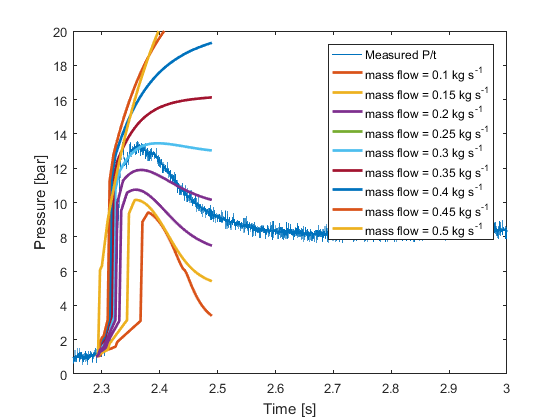
\includegraphics[width=\textwidth]{massflowrates}
		\caption{Pressure as a function of time for various mass--flow rates. Note that the lowest mass--flow rates are at the bottom, and the highest are at the top.}
		\label{fig:massflows}
	\end{figure}